\documentclass[../main.tex]{subfiles}
\begin{document}

\newpage
\section{Inferential statistics}

\subsection{Single-parameter linear regression}
Let $X$ denote the relative frequency of searches for the word "stocks", and let $Y$ denote the trading volume of the S\&P 500 index.
Performing linear regression between these two variables, with $X$ as the independent variable and $Y$ as the dependent variable, gives the line $Y = \hat{\beta} X + \hat{\alpha}$, where $\hat{\alpha} = 2.274 \times 10^9$ and $\hat{\beta} = 7.038 \times 10^7$.
Let us test the significance of this model at the $0.05$ significance level. We take the hypotheses
\begin{align*}
H_0: \beta = 0, \\
H_1: \beta \ne 0,
\end{align*}
but first check the Gauss-Markov conditions to show that the least-squares estimators are the best linear unbiased estimators.


To check the Gauss-Markov conditions, we will use the plots in Figures \ref{fig:sv-1}, \ref{fig:sv-2}, \ref{fig:sv-3}, \ref{fig:sv-4}.
The first plot shows that the expected value of the residuals is approximately $0$, regardless of the value predicted by linear regression. We therefore conclude that the expected values of the residuals are $0$, meaning that the first Gauss-Markov condition is satisfied.

Figure \ref{fig:sv-2} contains a Q-Q plot comparing the quantiles of the standardized residuals with those of the normal distribution. If the standardized residuals had a standard normal distribution, the points would follow the line $y = x$. Since the points lie approximately on a line through the origin, we can accept the assumption that the standardized residuals are normally distributed. A linear transformation of the residuals, specifically scaling, would produce a Q-Q plot with values lying on the line $y = x$. Since scaling a standard normal distribution produces a normal distribution centered at $0$, the assumption is justified.

The third plot shows that the square root of the absolute value of the standardized residuals is approximately constant, at least in the left half, where most of the data lie. We conclude that the variances of the residuals are approximately constant and consider the second Gauss-Markov condition satisfied.

It remains to discuss the lack of correlation between the residuals.
Since the data have a time component, we naturally expect observations to be correlated with those close to them in time.
Reducing the granularity of the data would reduce the correlation because the observations would be further apart in time, but in this paper we will use daily granularity.
We also justify the erratic nature of daily trading volume using the time series in Figure \ref{fig:volumen_timeseries}.

\begin{figure}[H]
    \centering
    \begin{minipage}{0.5\textwidth}
        \centering
        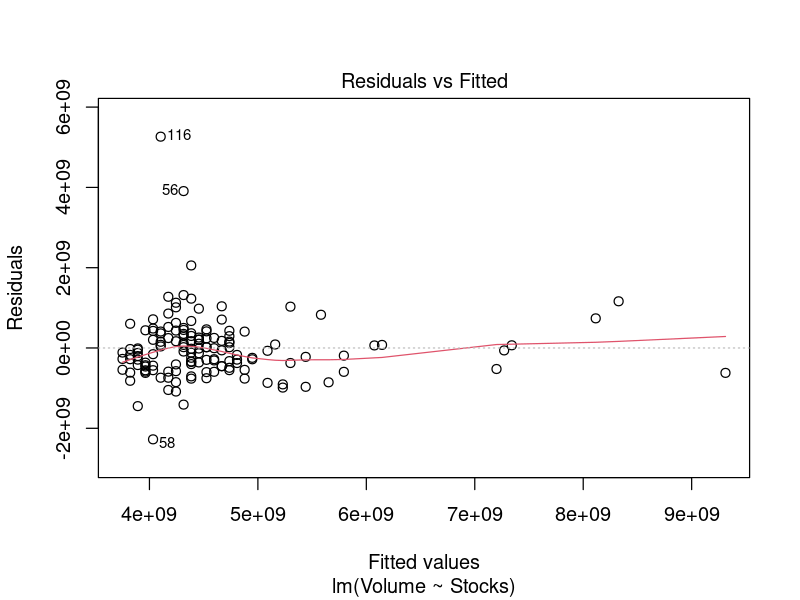
\includegraphics[width=\textwidth]{../lr/plots/Stocks-Volume_1.png}
        \caption{Relationship between $\widehat{Y}$ and the residuals}
        \label{fig:sv-1}
    \end{minipage}\hfill
    \begin{minipage}{0.5\textwidth}
        \centering
        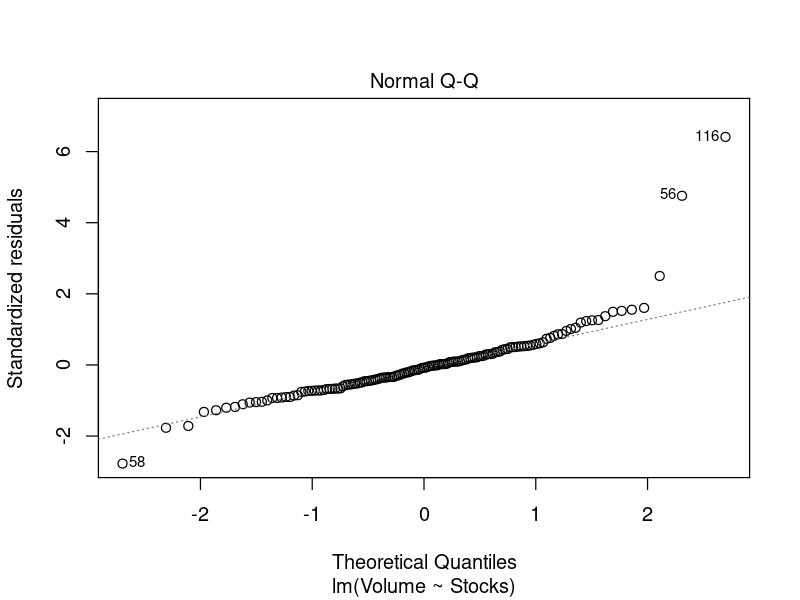
\includegraphics[width=\textwidth]{../lr/plots/Stocks-Volume_2.png}
        \caption{Q-Q plot of residuals}
        \label{fig:sv-2}
    \end{minipage}
    \begin{minipage}{0.5\textwidth}
        \centering
        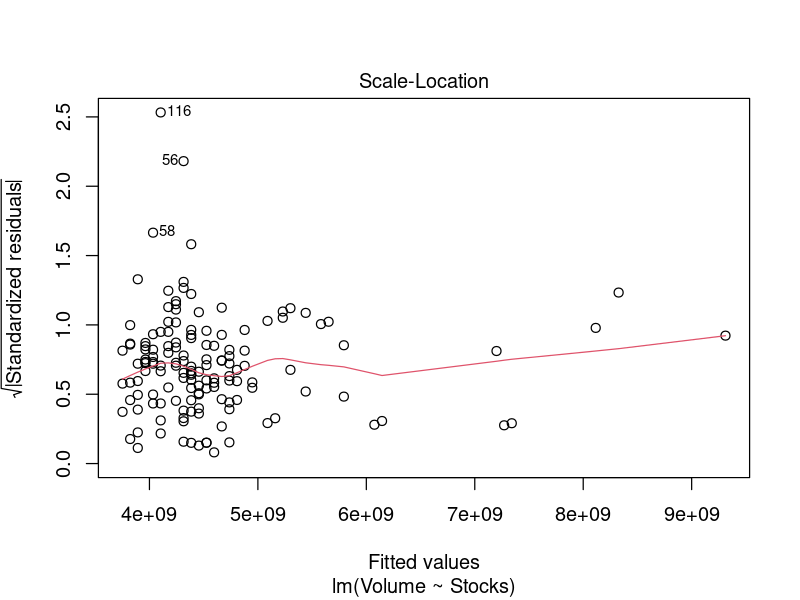
\includegraphics[width=\textwidth]{../lr/plots/Stocks-Volume_3.png}
        \caption{Relationship between $\widehat{Y}$ and the standardized residuals}
        \label{fig:sv-3}
    \end{minipage}\hfill
    \begin{minipage}{0.5\textwidth}
        \centering
        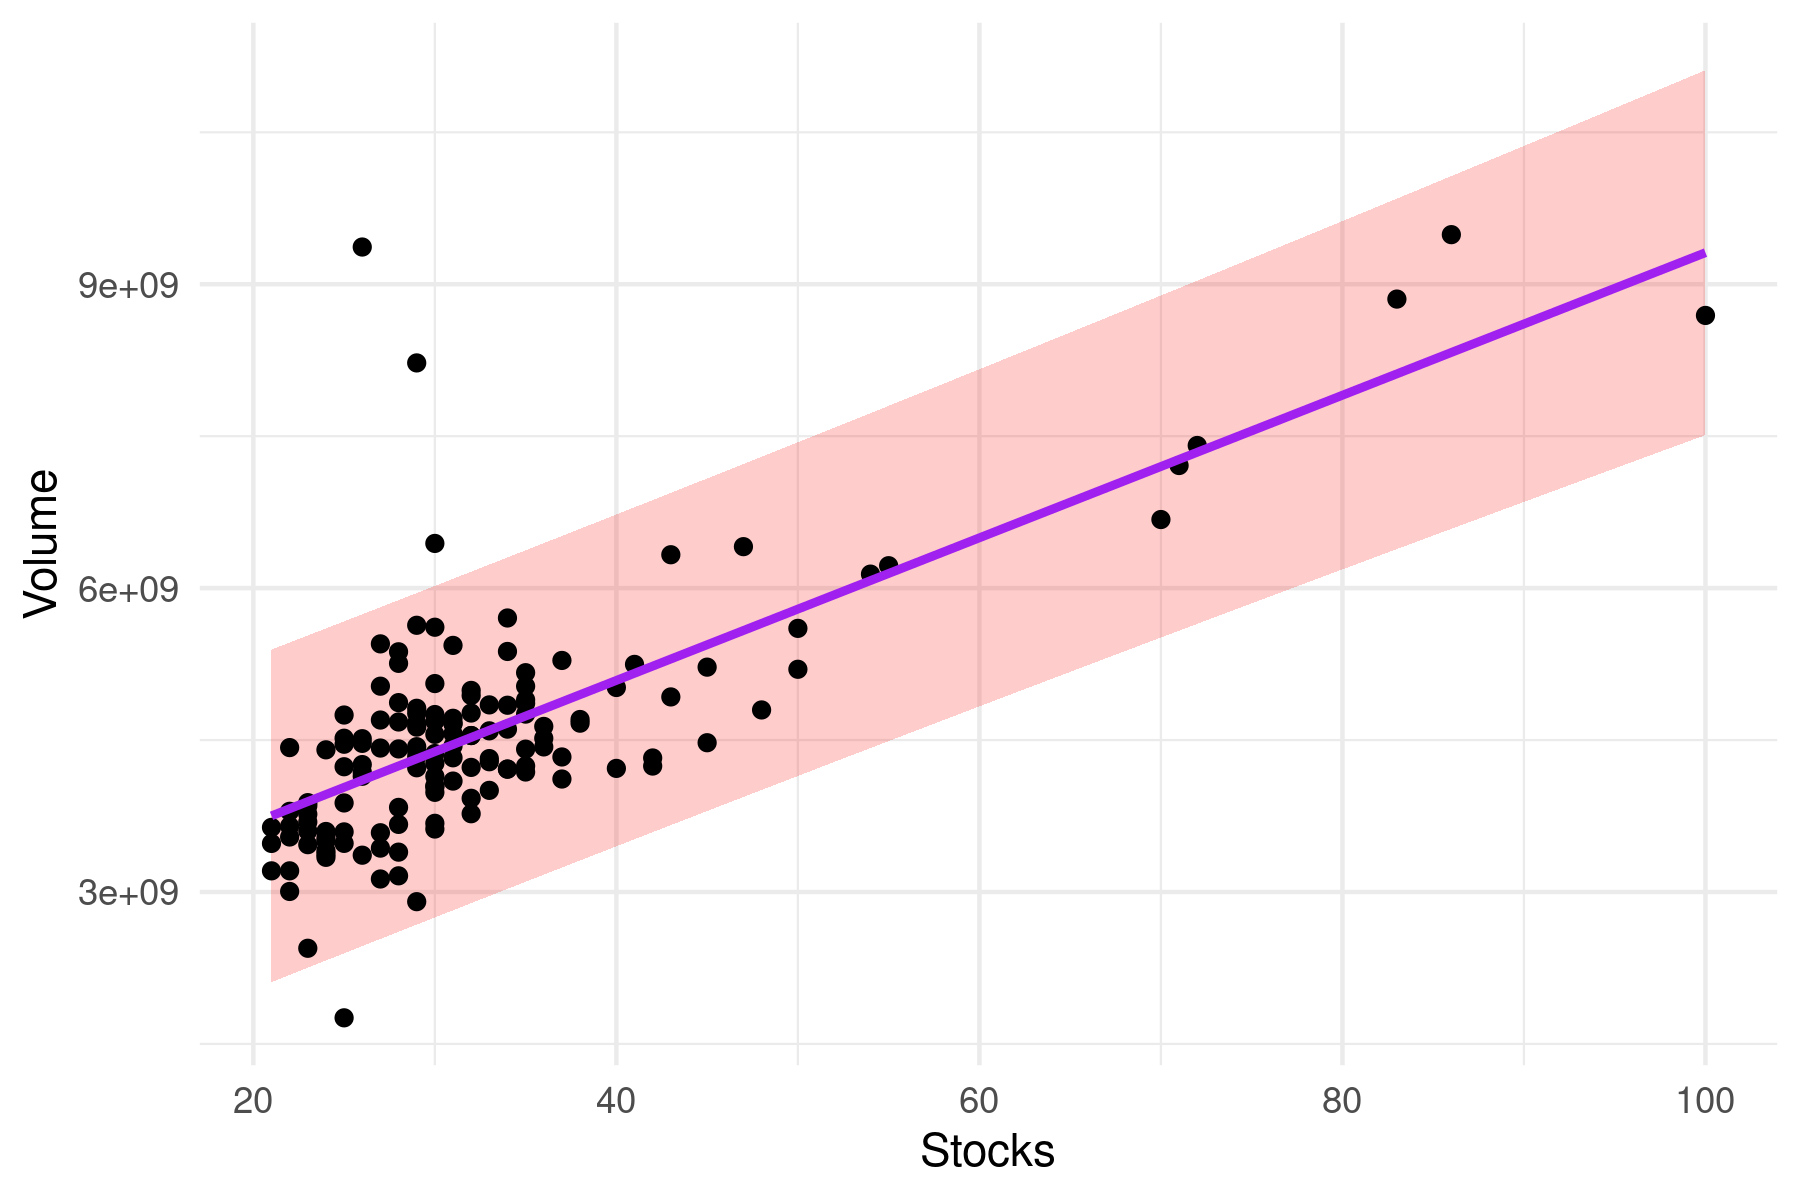
\includegraphics[width=\textwidth]{../lr/plots/Stocks-Volume_4.png}
        \caption{Linear regression line with a confidence interval}
        \label{fig:sv-4}
    \end{minipage}
\end{figure}


We can now construct a $95\%$ confidence interval for $\beta$ using the statistic
$$
\frac{\widehat{\beta} - \beta}{\widehat{\sigma} \cdot \sqrt{\frac{1}{S_{xx}}}} \sim t(n-2).
$$
The resulting interval is \newline
$[5.9165060 \times 10^7, 8.1599495 \times 10^7]$. This also leads us to conclude that the linear regression is statistically significant at the $0.05$ level, since $0$ is not within this interval; we reject the hypothesis $H_0$.
For $\alpha$, the $95\%$ confidence interval is $[1.880536685 \times 10^9, 2.666848278 \times 10^9]$.

Figure \ref{fig:sv-4} illustrates the linear model with confidence intervals. We justify the relatively close fit of the data to the linear model by the substantial $R^2$ value of $0.5218$ and the high Pearson correlation coefficient in Table \ref{fig:correlation_matrix}.
It is interesting to note that the most notable outlier, observation $116$, occurred on 21.03.2025., the day Trump announced that he would present a new tariff strategy on "Liberation Day".

\begin{figure}[H]
    \centering
    \begin{minipage}{0.5\textwidth}
        \centering
        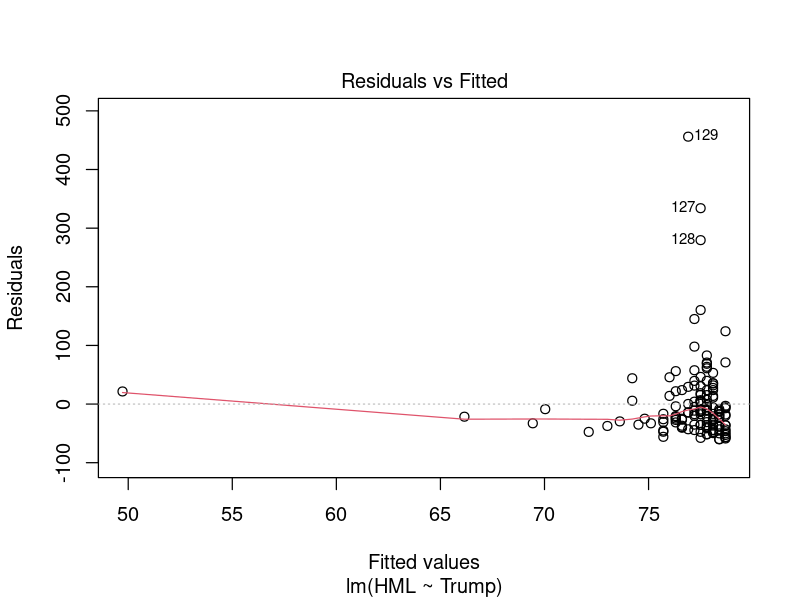
\includegraphics[width=\textwidth]{../lr/plots/Trump-Volatility_1.png}
        \caption{Relationship between $\widehat{Y}$ and the residuals}
        \label{fig:tv-1}
    \end{minipage}\hfill
    \begin{minipage}{0.5\textwidth}
        \centering
        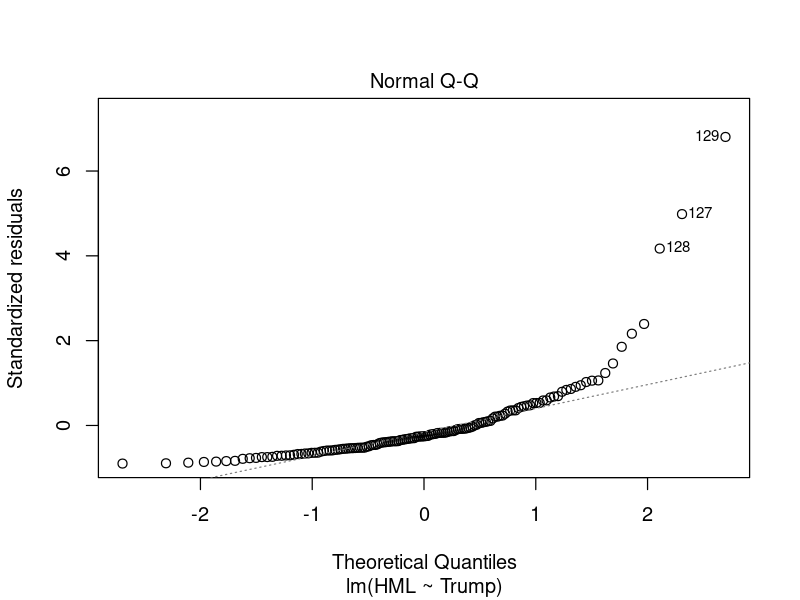
\includegraphics[width=\textwidth]{../lr/plots/Trump-Volatility_2.png}
        \caption{Q-Q plot of residuals}
        \label{fig:tv-2}
    \end{minipage}
    \begin{minipage}{0.5\textwidth}
        \centering
        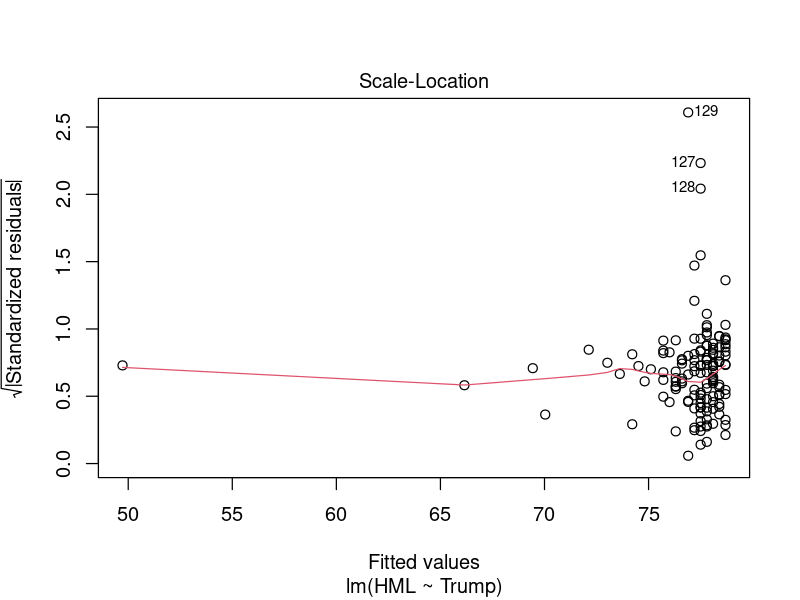
\includegraphics[width=\textwidth]{../lr/plots/Trump-Volatility_3.png}
        \caption{Relationship between $\widehat{Y}$ and the standardized residuals}
        \label{fig:tv-3}
    \end{minipage}\hfill
    \begin{minipage}{0.5\textwidth}
        \centering
        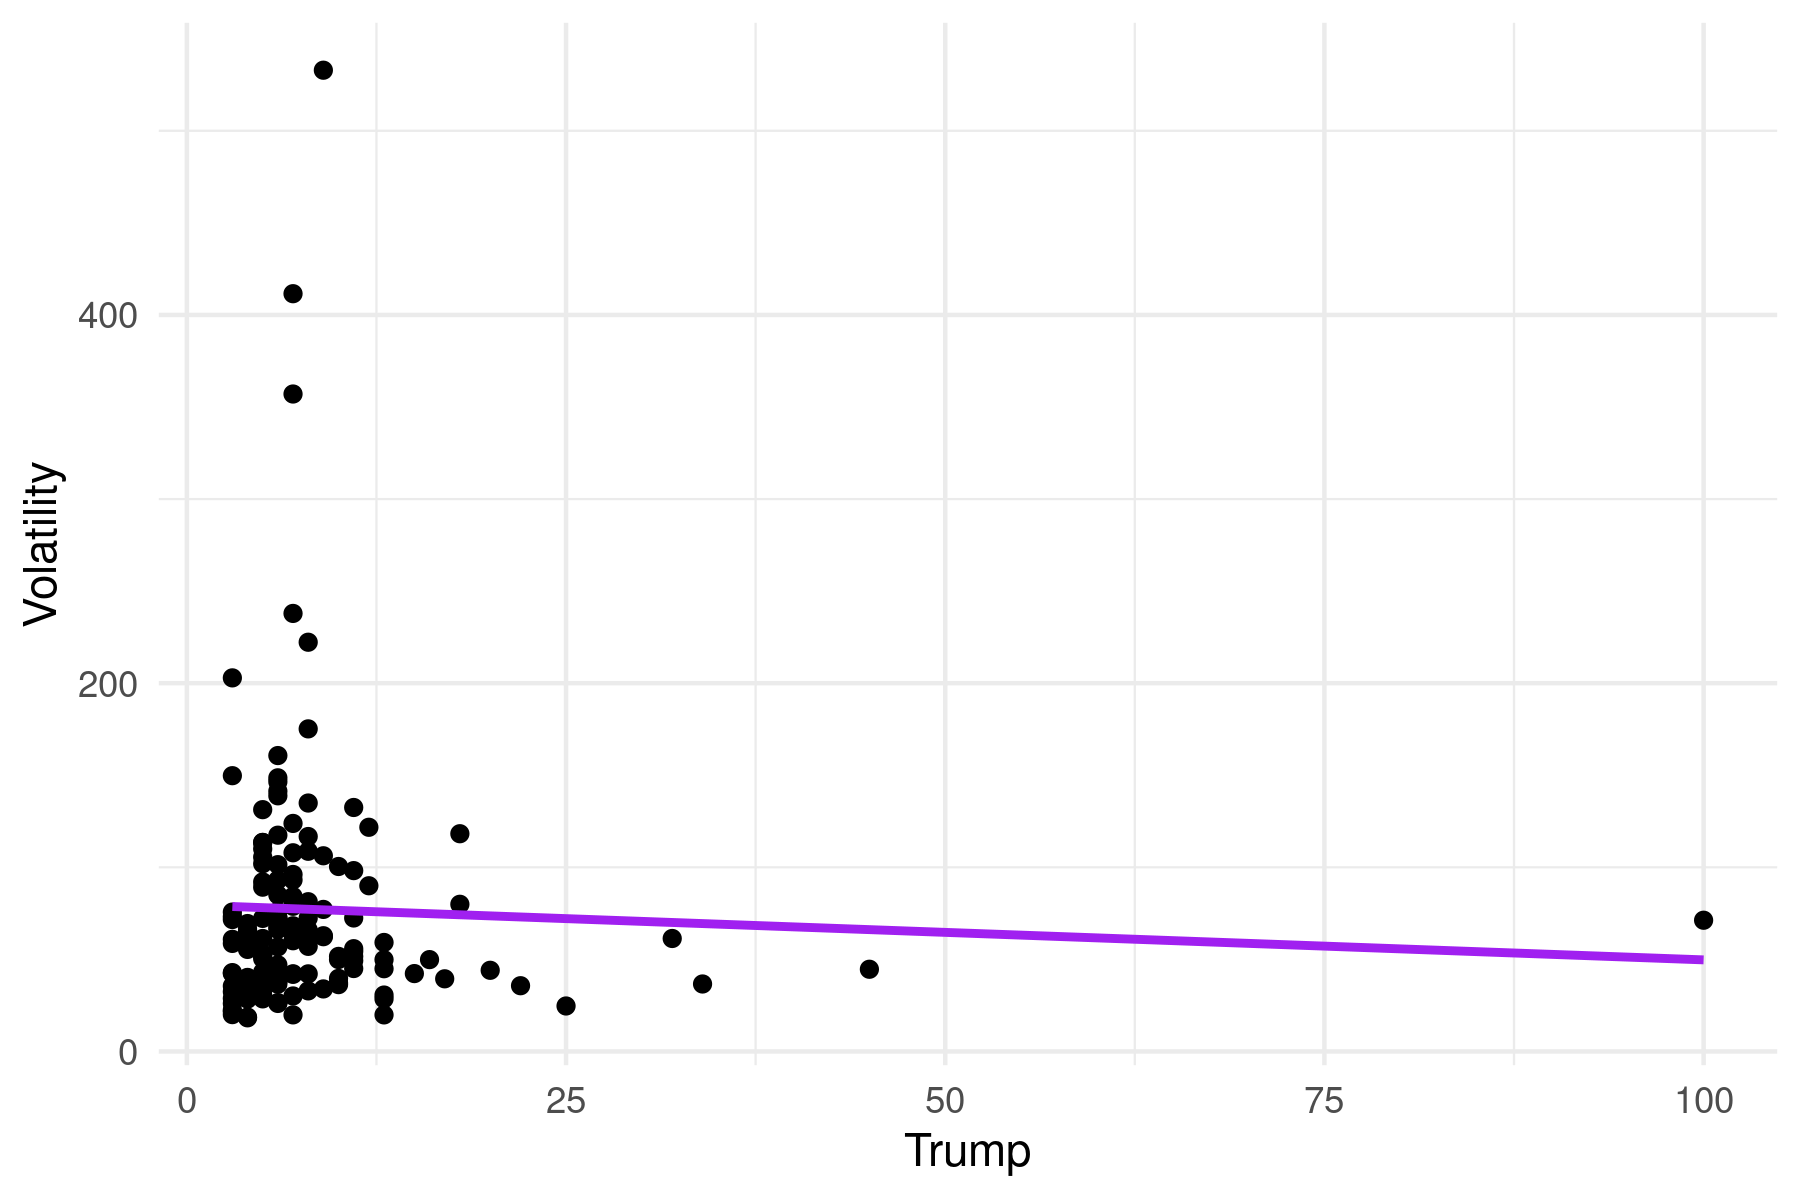
\includegraphics[width=\textwidth]{../lr/plots/Trump-Volatility_4.png}
        \caption{Linear regression line}
        \label{fig:tv-4}
    \end{minipage}\hfill
\end{figure}
Let us now consider the dependence of HML on "Trump". From the plots in Figures \ref{fig:tv-1}, \ref{fig:tv-2}, \ref{fig:tv-3}, \ref{fig:tv-4},
we see that the Gauss-Markov conditions are not satisfied.
The expected value of the residuals decreases substantially at high values predicted by the linear model, and the Q-Q plot does not resemble a line through the origin at all. Nevertheless, Figure \ref{fig:tv-4} suggests that it makes more sense to perform linear regression between the logarithms of the two variables, since both variables have "long tails" that can be tamed using logarithms.

\begin{figure}[H]
    \centering
    \begin{minipage}{0.5\textwidth}
        \centering
        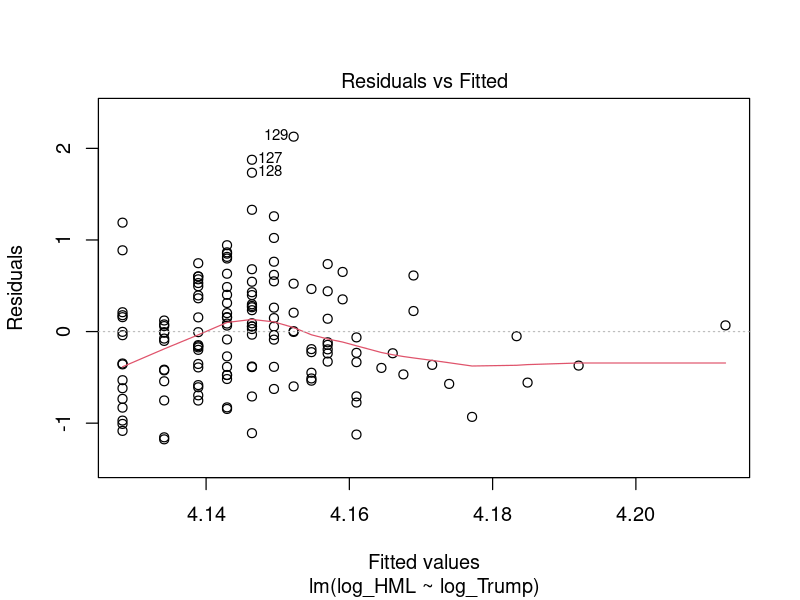
\includegraphics[width=\textwidth]{../lr/plots/log_Trump-log_Volatility_1.png}
        \caption{Relationship between $\widehat{Y}$ and the residuals}
        \label{fig:ltlv-1}
    \end{minipage}\hfill
    \begin{minipage}{0.5\textwidth}
        \centering
        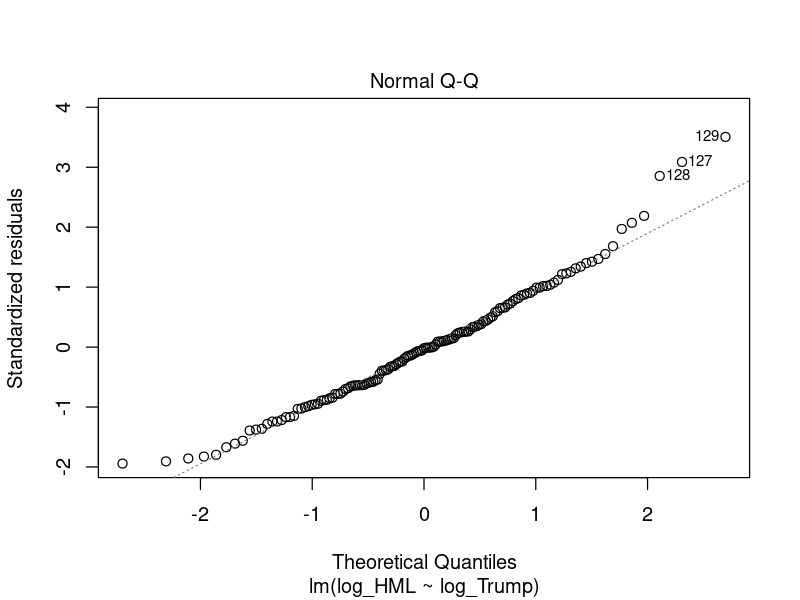
\includegraphics[width=\textwidth]{../lr/plots/log_Trump-log_Volatility_2.png}
        \caption{Q-Q plot of residuals}
        \label{fig:ltlv-2}
    \end{minipage}
    \begin{minipage}{0.5\textwidth}
        \centering
        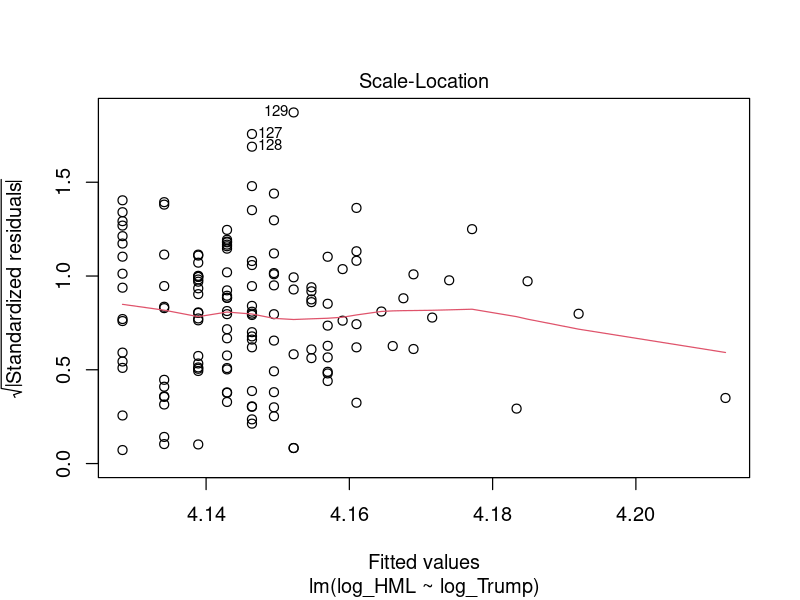
\includegraphics[width=\textwidth]{../lr/plots/log_Trump-log_Volatility_3.png}
        \caption{Relationship between $\widehat{Y}$ and the standardized residuals}
        \label{fig:ltlv-3}
    \end{minipage}\hfill
    \begin{minipage}{0.5\textwidth}
        \centering
        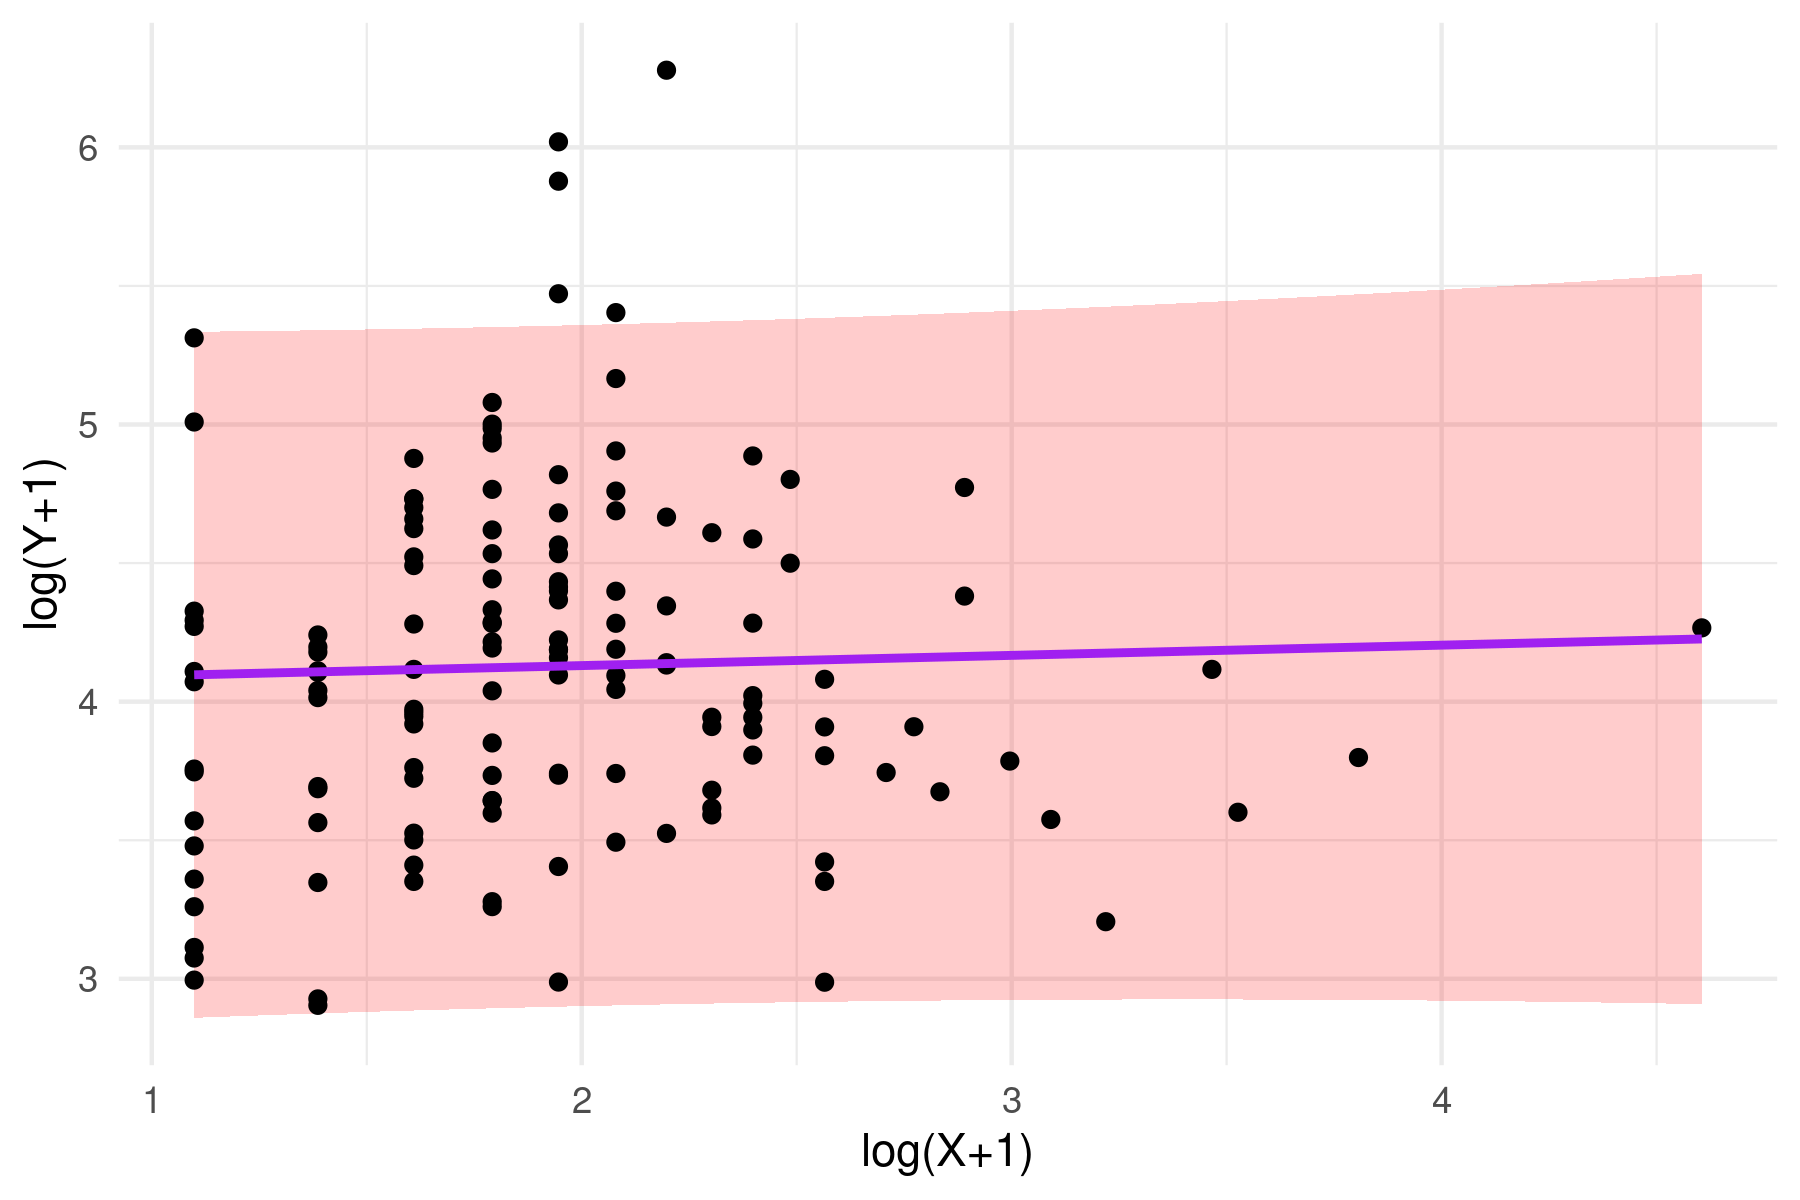
\includegraphics[width=\textwidth]{../lr/plots/log_Trump-log_Volatility_4.png}
        \caption{Linear regression line}
        \label{fig:ltlv-4}
    \end{minipage}\hfill
\end{figure}
Indeed, from the plots in Figures \ref{fig:ltlv-1}, \ref{fig:ltlv-2}, \ref{fig:ltlv-3}, \ref{fig:ltlv-4},
we see that the Gauss-Markov conditions are closer to being satisfied, so we can expect the estimators obtained by linear regression to be better.
Linear regression gives $\log(Y + 1) = \hat{\beta} \log(X + 1) + \hat{\alpha}$, where $\hat{\beta} = 0.02607$ and $\hat{\alpha} = 4.0921$.
To check the significance of this linear regression, we construct a $95\%$ confidence interval for $\beta$, $[-0.1703286, 0.2224685]$, and observe that $0$ lies within it. Moreover, the $90\%$ confidence interval is $[-0.138419, 0.1995589]$, so even at the $0.10$ level we cannot reject the hypothesis $H_0: \beta = 0$ in favor of $H_1: \beta \ne 0$.

Let us pay particular attention to this last result: we cannot obtain a statistically significant estimate of volume using only data on the frequency of searches for the word "Trump".
In the next section, we will see how this changes when we add another regressor to the linear model.

\subsection{Multiple linear regression}

We now perform multiple regression with the independent variables ``Trump" ($X_1$) and ``Stocks" ($X_2$), and the dependent variable hml ($Y$).

Performing linear regression gives the relationship $Y = \hat{\alpha} + \hat{\beta}_1 X_1 + \hat{\beta}_2 X_2$, with $\hat{\alpha} = -50.77$, $\hat{\beta}_1 = -1.08$, $\hat{\beta}_2 = 4.17$. We will test the model at the $0.05$ significance level, and can now consider two sets of hypotheses:
\begin{align*}
	H_0^1&: \beta_1 = 0, \\
	H_1^1&: \beta_1 \neq 0 \\
	H_0^2&: \beta_2 = 0, \\
	H_1^2&: \beta_2 \neq 0.
\end{align*}

We construct $95\%$ confidence intervals for $\beta_1, \beta_2$ in the same way as in the single-parameter case. For $\beta_1$, we obtain $[-1.858206, -0.308047]$, and for $\beta_2$, $[3.557971, 4.784710]$.

Neither the interval for $\beta_1$ nor the interval for $\beta_2$ contains zero. We conclude that we can reject both null hypotheses, meaning that in multiple regression, hml depends on both ``Trump" and ``Stocks", although this was not the case in single-parameter regression. Slightly modified hypotheses are often used in multiple regression:

\begin{align*}
	H_0'&: \beta_1 = \beta_2 = 0, \\
	H_1'&: \beta_1 \neq 0 \lor \beta_2 \neq 0.
\end{align*}

Our alternative hypotheses are strictly stronger than this one, in the sense that if we reject our null hypotheses $H_0^1, H_0^2$, we necessarily also reject the null hypothesis $H_0'$. Thus, the preceding analysis also allows us to reject this null hypothesis. The interpretation is that performing regression was meaningful overall, since $Y$ depends on the independent variables being examined.

In particular, looking only at $\hat{\beta}_1$, the coefficient of the variable ``Trump", we see that it is significant and negative. Thus, when the additional variable ``Stocks" is taken into account, ``Trump" becomes a significant predictor of hml, although it was not significant in the single-parameter case. Since the coefficient is negative, ``Trump" and hml are inversely related. This is somewhat surprising, but we obtained a similar result (although not significant) in the previous section.

The $95\%$ confidence interval for $\alpha$ is $[-72.344428, -29.192035]$.

The $R^2$ value is $0.5644$. We have obtained a relatively good model for the data, for example compared with the models from single-parameter regression. Visualizing regression with two parameters is clearly more difficult, but we can still interpret it through Figure \ref{fig:multipar}, which shows a relatively good relationship between the data and the model.

\begin{figure}[H]
    \centering
	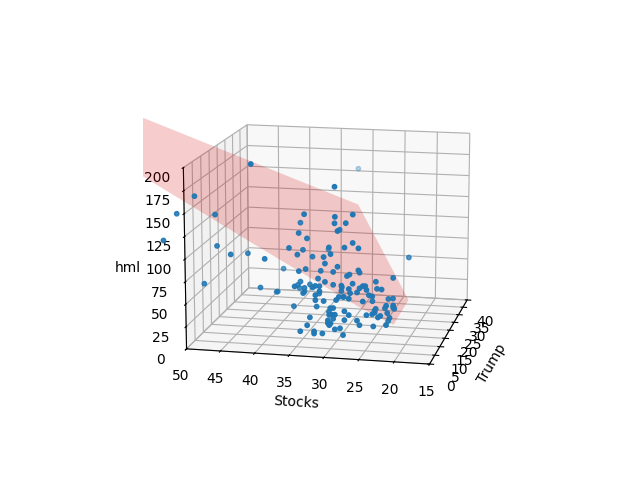
\includegraphics[width=0.8\textwidth]{../plots/multipar2.png}
	\caption{Multiple regression of the variables ``Trump", ``Stocks", and hml.}
	\label{fig:multipar}
\end{figure}

\subsection{Kolmogorov-Smirnov test}

We will use the Lilliefors version of the Kolmogorov-Smirnov test to check the distribution of hml. In Figure \ref{fig:hml_fitted}, the distribution appears log-normal; of all the variables examined, this histogram most strongly suggests a log-normal distribution. We therefore aim to test this claim at the $0.05$ significance level. Let $Y$ denote hml. We test the hypotheses:

\begin{align*}
	H_0&: \log{Y} \sim N(\mu, \sigma) \\
	H_1&: \log{Y} \textrm{ does not have a normal distribution.}
\end{align*}

Applying the test to $\log{Y}$ gives $D = 0.05849$ and $p = 0.2701$. Since $p > 0.05$, we cannot reject the null hypothesis that $Y$ is log-normally distributed.

Let us apply the Lilliefors version of the Kolmogorov-Smirnov test to another example. Figure \ref{fig:promjena_fitted} suggests that change has a somewhat normal distribution. Denote it by $X$ and test the hypothesis at the $0.05$ significance level

\begin{align*}
	H_0&: X \sim N(\mu, \sigma) \\
	H_1&: X \textrm{ does not have a normal distribution.}
\end{align*}

We obtain $D = 0.1148$ and $p = 8.739 \times 10^{-5}$. Since $p < 0.05$, we reject the null hypothesis and conclude that change is not normally distributed.

In general, examining other analyses based on much larger datasets suggests that the tails of the distribution of change are considerably heavier than those of a normal distribution. In our data, this is particularly apparent because of the outlier corresponding to the reciprocal tariffs.

\end{document}
